\documentclass[11pt]{article}

\usepackage{amsmath}
\usepackage{amssymb}
\usepackage{my-acronyms}
\usepackage{hyperref}
\usepackage{tikz}

\title{
    Intelligent System 2\\
    Tutorial week 11: Abstract Argumentation
}

\author{
    Matteo Magnini\\
    \href{mailto:matteo.magnini@uni.lu}{matteo.magnini@uni.lu}
}

\date{
    7 May, 2026
}

\begin{document}

\maketitle

\section{Exercises}

\subsection{Exercise 1: Conflict-free Sets}

Consider the argumentation framework $AF = (AR, \to)$:

\begin{center}
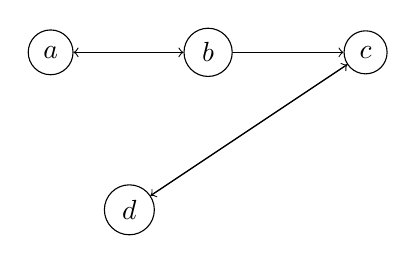
\begin{tikzpicture}
\node[circle,draw] (a) at (0,0) {$a$};
\node[circle,draw] (b) at (2,0) {$b$};
\node[circle,draw] (c) at (4,0) {$c$};
\node[circle,draw] (d) at (1,-2) {$d$};

\path[->]
(a) edge (b)
(b) edge (a)
(b) edge (c)
(c) edge (d)
(d) edge (c);
\end{tikzpicture}
\end{center}

\begin{enumerate}
    \item List \textbf{all} conflict-free sets.
    \item Which of them are $\subseteq$-maximal?
\end{enumerate}

\subsection{Exercise 2: Naive vs Non-naive}

Using the same framework as Exercise 1:

\begin{enumerate}
    \item Compute all \textbf{naive extensions}.
    \item Give an example of a conflict-free set that is \textbf{not} naive.
\end{enumerate}

\subsection{Exercise 3: Defence and Admissibility}

Consider the argumentation framework:

\begin{center}
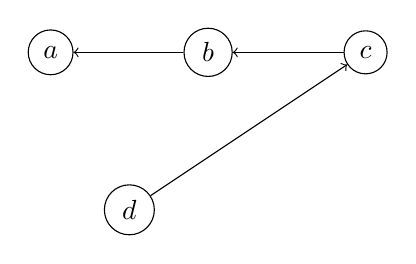
\begin{tikzpicture}
\node[circle,draw] (a) at (0,0) {$a$};
\node[circle,draw] (b) at (2,0) {$b$};
\node[circle,draw] (c) at (4,0) {$c$};
\node[circle,draw] (d) at (1,-2) {$d$};

\path[->]
(b) edge (a)
(c) edge (b)
(d) edge (c);
\end{tikzpicture}
\end{center}

\begin{enumerate}
    \item Does $\{a\}$ defend $a$?
    \item Does $\{c\}$ defend $c$?
    \item Find all \textbf{admissible} sets.
\end{enumerate}

\subsection{Exercise 4: Complete Extensions}

Using the same framework as Exercise 3:

\begin{enumerate}
    \item Compute all admissible sets.
    \item Among them, identify the \textbf{complete extensions}.
    \item Explain why some admissible sets are not complete.
\end{enumerate}

\subsection{Exercise 5: Grounded Extension (Procedure)}

Consider the following framework:

\begin{center}
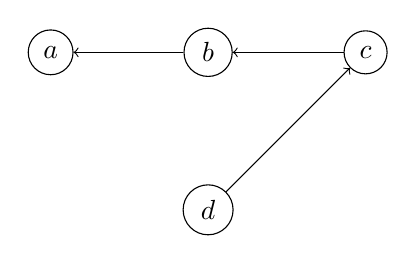
\begin{tikzpicture}
\node[circle,draw] (a) at (0,0) {$a$};
\node[circle,draw] (b) at (2,0) {$b$};
\node[circle,draw] (c) at (4,0) {$c$};
\node[circle,draw] (d) at (2,-2) {$d$};

\path[->]
(b) edge (a)
(c) edge (b)
(d) edge (c);
\end{tikzpicture}
\end{center}

\textbf{Recall (slides):}
Grounded labelling procedure:
\begin{enumerate}
    \item All arguments start \textbf{yellow} (undecided).
    \item Mark as \textbf{green} (accepted) every argument that is \emph{not attacked} by any green or yellow argument.
    \item Mark as \textbf{red} (rejected) every argument attacked by a green one.
    \item Iterate until no change occurs.
\end{enumerate}

\subsection{Exercise 6: Preferred vs Complete}

Consider:

\begin{center}
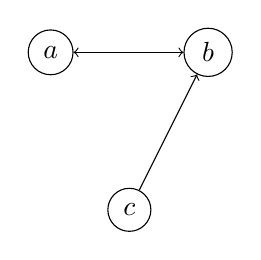
\begin{tikzpicture}
\node[circle,draw] (a) at (0,0) {$a$};
\node[circle,draw] (b) at (2,0) {$b$};
\node[circle,draw] (c) at (1,-2) {$c$};

\path[->]
(a) edge (b)
(b) edge (a)
(c) edge (b);
\end{tikzpicture}
\end{center}

\begin{enumerate}
    \item Compute all complete extensions.
    \item Compute all preferred extensions.
    \item Which preferred extensions are not grounded?
\end{enumerate}

\subsection{Exercise 7: Stable Semantics}

Consider:

\begin{center}
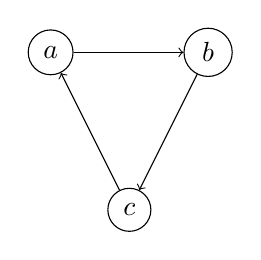
\begin{tikzpicture}
\node[circle,draw] (a) at (0,0) {$a$};
\node[circle,draw] (b) at (2,0) {$b$};
\node[circle,draw] (c) at (1,-2) {$c$};

\path[->]
(a) edge (b)
(b) edge (c)
(c) edge (a);
\end{tikzpicture}
\end{center}

\begin{enumerate}
    \item Find all stable extensions.
    \item Does a stable extension always exist? Explain using this example.
\end{enumerate}

\subsection{Exercise 8: Full Practice (Mini Homework)}

Consider:

\begin{center}
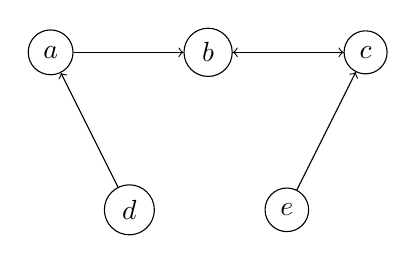
\begin{tikzpicture}
\node[circle,draw] (a) at (0,0) {$a$};
\node[circle,draw] (b) at (2,0) {$b$};
\node[circle,draw] (c) at (4,0) {$c$};
\node[circle,draw] (d) at (1,-2) {$d$};
\node[circle,draw] (e) at (3,-2) {$e$};

\path[->]
(a) edge (b)
(b) edge (c)
(c) edge (b)
(d) edge (a)
(e) edge (c);
\end{tikzpicture}
\end{center}

\begin{enumerate}
    \item Find:
    \begin{itemize}
        \item one naive extension
        \item one complete extension
        \item the grounded extension
        \item one preferred extension
        \item one stable extension (if it exists)
    \end{itemize}

    \item Are any of them equal? Explain.
\end{enumerate}

\end{document}